\documentclass[article,	12pt, oneside, 	a4paper, english, brazil
%,sumario=tradicional
]{abntex2}
\linespread{1.3}

\usepackage[brazilian,hyperpageref]{backref}	 % Paginas com as citações na bibl
\usepackage[alf,abnt-emphasize=bf,abnt-etal-list=5]{abntex2cite} % Padrao de citacao alfabetico e com destaque em negrito
\usepackage{amsmath}
\usepackage{lmodern}			% Usa a fonte Latin Modern
\usepackage[T1]{fontenc}		% Selecao de codigos de fonte.
\usepackage[utf8]{inputenc}		% Codificacao do documento (conversão automática dos acentos)
\usepackage{indentfirst}		% Indenta o primeiro parágrafo de cada seção.
\usepackage{nomencl} 			% Lista de simbolos
\usepackage{color}				% Controle das cores
\usepackage{graphicx}			% Inclusão de gráficos
\usepackage{microtype} 			% para melhorias de justificação
\usepackage{enumitem}
\usepackage{wasysym}
\usepackage{amssymb}
\usepackage{verbatim}
\usepackage{dsfont}
\usepackage{textcomp}
\usepackage{pstricks}
\usepackage{pstricks-add}
\usepackage[normalem]{ulem} 
\usepackage{indentfirst}
\usepackage{color}
\usepackage{array}
\usepackage{pst-3dplot}
\usepackage[bottom=2.5cm,a4paper,hmargin={3cm,2cm}]{geometry}
\usepackage{multirow}
\usepackage{bigstrut}
\usepackage{float}
\usepackage{hyperref}
\usepackage{pdfpages}
\hypersetup{hidelinks,
            linkcolor = blue} % Changes the link color to black and hides the hideous red border that usually is created
   


% Configurações do pacote backref
% Usado sem a opção hyperpageref de backref
\renewcommand{\backrefpagesname}{Citado na(s) página(s):~}
% Texto padrão antes do número das páginas
\renewcommand{\backref}{}
% Define os textos da citação
\renewcommand*{\backrefalt}[4]{%
	\ifcase #1 %
		Nenhuma citação no texto.%
	\or%
		Citado na página #2.%
	\else%
		Citado #1 vezes nas páginas #2.%
	\fi%
}%
% ---

\makeatletter
\hypersetup{
     	%pagebackref=true,
		pdftitle={\@title}, 
		pdfauthor={\@author},
    	pdfsubject={\imprimirpreambulo},
	    pdfcreator={LaTeX with abnTeX2},
		pdfkeywords={TCC}, 
		colorlinks=true,       		% false: boxed links; true: colored links
    	linkcolor=black,          	% color of internal links
    	citecolor=black,        		% color of links to bibliography
    	filecolor=black,      		% color of file links
		urlcolor=black,
		bookmarksdepth=4
}
\makeatother



\addto\captionsbrazil{
\renewcommand{\anexosname}{\textbf{ANEXOS}}
\renewcommand{\apendicesname}{\textbf{APÊNDICES}}
\renewcommand{\bibname}{Refer\^encias Bibliográficas}
}

% -----------------------------------------------------------------------------
% CONFIGURACAO DO SUMARIO
% -----------------------------------------------------------------------------

\setlength\cftbeforechapterskip{0pt}

\renewcommand{\ABNTEXchapterfont}{\bfseries}
\renewcommand{\ABNTEXchapterfontsize}{\normalsize}
%\setboolean{ABNTEXupperchapter}{false}


\renewcommand{\ABNTEXsectionfontsize}{\normalsize}
\renewcommand{\ABNTEXsubsectionfont}{\itshape}
\renewcommand{\ABNTEXsubsectionfontsize}{\normalsize}
\renewcommand{\cftsubsectionfont}{\normalfont}
\renewcommand{\cftsubsectionfont}{\itshape}
%\renewcommand{\tocheadstart}{\ABNTEXchapterfont}
\renewcommand{\tocheadstart}{\ABNTEXsectionfont}

\DeclareMathOperator{\sen}{sen}
%\renewcommand{\ABNTchapterfont}{\bfseries}

 
 
\makepagestyle{meuestilo}
\makeevenhead{meuestilo}{\ABNTEXfontereduzida\thepage}{}{}
\makeoddhead{meuestilo}{}{}{\ABNTEXfontereduzida\thepage}


\renewcommand{\bibsection}{%
    \chapter*{\bibname}
    \bibmark
    \ifnobibintoc\else
    \phantomsection
    \addcontentsline{toc}{chapter}{{\bibname}}
    \fi
    \prebibhook
}

 
% Coloca a citação de equação, \autoref{label}, no formato Equação (2.1)
%\def\equationautorefname~#1\null{Equa\c c\~ao~(#1)\null}
% % % % % % % % % % % % % % % % % % % % % % % % % % % % % % % % % % % %  
 
\usepackage{listings}


\begin{document}
\pagestyle{meuestilo}

\begin{capa}

    \begin{center}
        {\MakeUppercase{\Large Universidade de São Paulo}}\\
        {\MakeUppercase{\large Dep. de Ciências da Computação}}\\
        {\MakeUppercase{\large SCC0640 - Bases de Dados}}

        \vspace{2cm}

        \begin{flushright}
            Elaine Parros Machado de Souza
        \end{flushright}


        \vspace{4cm}

        {\MakeUppercase{\large Auxílio a Dependentes Químicos e Moradores de Rua}}
        \\[0.125cm]
        {\MakeUppercase {\normalsize Projeto de Base de Dados - SCC0640 }}\\[3cm]
    \end{center}

    \begin{flushright}
        {\large	Emanuel Lace Aranha, n\textdegree ~11234224}\\
        {\large	Felipe de Alcantara Tomé, n\textdegree ~11800970}\\
        {\large	Francisco Reis Nogueira, n\textdegree ~11954374}\\
        {\large	Joao Augusto Fernandes Barbosa, n\textdegree ~11953348}\\

    \end{flushright}

    \begin{center}
        \vfill
        São Carlos \\
        \the\year  % imprime o ano

    \end{center}
\end{capa}

% Lista de figuras. Se o relatório não tiver figuras, colocar % no início das duas linhas a seguir
% \pdfbookmark[0]{\listfigurename}{lof}
% \listoffigures*
%\cleardoublepage
% ---

\vspace{3cm}

% Lista de figuras. Se o relatório não tiver tabelas, colocar % no início das duas linhas a seguir
%\pdfbookmark[0]{\listtablename}{lot}
%\listoftables*
%\cleardoublepage

% Lista de Conteúdo (sumário).
\pdfbookmark[0]{\contentsname}{toc}
\tableofcontents*
\cleardoublepage



\section{Introdução}
\label{sec:introducao}
Uma das principais problemáticas encaradas dentro do contexto sociopolítico urbano, principalmente dentro de megalópoles, é a gritante desigualdade encontrada por entre as entranhas de suas ruas, ocasionando em uma quantidade gritante de cidadãos sem acesso ao básico para sua sobrevivência. A origem desta situação é, por muitas vezes, definida erroneamente como vinda da dependência química, entretanto os motivos são diversos mas, fato é, que em regiões específicas de grandes centros urbanos existe uma concentração enorme de pessoas sem moradia fixa que fazem uso de algum entorpecente com frequência. Este quadro força que a abordagem de acolhimento em abrigos e em assistências comunitárias tenham maior sensibilidade quanto a isso, necessitando a observação dos dados de evolução do auxiliado, dos recursos financeiros, dos voluntários e das campanhas de auxílio.

O seguinte projeto se trata de uma iniciativa dos moradores do centro de uma grande metrópole para reestruturação da região da forma mais humanizada possível, essencialmente teremos um \textbf{auxiliado}, o qual será recebido por este coletivo, classificado por auto-declaração e atendido da forma mais personalizada possível.


\section{Levantamento de requisitos}

\subsection{Descrição da aplicação prática da base de dados}
A entidade principal desta base será o \textbf{auxiliado}, representando o \textbf{morador de rua} e/ou \textbf{dependente químico} assistido, pois ele será o ponto focal do projeto, o qual possui todos os identificadores comuns de um cidadão brasileiro como \textbf{CPF}, desta forma o \textbf{funcionário} da ação social poderá registrar todas as informações pessoais e específicas através desta chave identificadora, e.g, algum tipo de formação ou \textbf{habilidade} profissional, \textbf{idade}, a qual será um atributo derivado de \textbf{Data de nascimento}, \textbf{sexo}, \textbf{nome} e, caso aplicável, \textbf{local} de moradia fixo. Isto é feito para que as \textbf{frentes} do projeto consigam se organizar a fim de encaminhar o \textbf{auxiliado} para os programas de \textbf{reestruturação profissional} em \textbf{empresas parceiras} e de \textbf{reestruturação social} em \textbf{clínicas} com sensibilidade geográfica, de faixa etária e de lotação das instituições pois elas possuem um \textbf{número máximo de pacientes e funcionários}, a fim de funcionar corretamente e promover uma reerguida confortável aos auxiliados. Ademais, a generalização feita através desta entidade faz com que ocorra uma simplificação quando é necessário atribuir os \textbf{auxiliados} a programas focalizados, referenciando apenas as entidades específicas \textbf{dependente químico} e \textbf{morador de rua}, possibilitando a classificação de ambos através do atributo multi-valorado \textbf{tipo}.

As instalações físicas da ação com \textbf{local} fixo, chamadas de \textbf{centros comunitários}, são pontos organizacionais que se encarregam de administrar o próprio fluxo financeiro através do atributo \textbf{caixa}, representando todo o dinheiro atualmente em posse do \textbf{centro comunitário}. Todo centro tem o próprio \textbf{presidente}, representado pela relação \textbf{preside} entre \textbf{funcionário} e \textbf{centro comunitário}, seus funcionários participantes representados pela relação \textbf{participa}, \textbf{CNPJ} único e as frentes que são administradas por ele. De forma que, cada \textbf{centro comunitário} realiza seus próprios eventos beneficentes com \textbf{data}, \textbf{hora} e \textbf{local} específicos, além de campanhas de subsídio de produtos de uso pessoal através da \textbf{tesouraria}. 

Os casos de dependência química são tratados através da internação não compulsória do auxiliado em \textbf{clínicas} parceiras que promovam programas de \textbf{reabilitação}, caso ela aconteça se faz interessante manter a \textbf{presença} do \textbf{auxiliado}, assim como a \textbf{data} de início do tratamento. Por questões organizacionais e de respaldo legal, toda \textbf{clínica} deve ter um \textbf{CNPJ} válido, um \textbf{nome} e ter em registro seu \textbf{número total de funcionários e pacientes}(atributos \textbf{NuFuncionarios} e \textbf{NuPacientes}), vale ressaltar que a \textbf{clínica} não recebe somente pacientes dos \textbf{centros comunitários}.

Todos os \textbf{auxiliados} tem a possibilidade de ingressar em um esquema de \textbf{emprego supervisionado} caso queiram, estes acordos são firmados entre os ingressantes e as \textbf{empresas parceiras} com a ajuda da frente de \textbf{reestruturação profissional}. Os auxiliados são contratados caso o numero máximo de funcionários (atributo \textbf{MaxFuncionarios}) das empresas parceiras seja diferente do número atual de funcionários (atributo \textbf{NuFuncionarios}) e conforme o interesse da empresa.

O projeto possui acordo com ONG's, que oferecem especificamente alojamento temporário para os \textbf{moradores de rua} assistidos pelo projeto, representado pelo relacionamento \textbf{aloja}. Além das relações específicas dos \textbf{terceiros} supracitadas, todas as especificações desta classe generalizada, incluindo qualquer \textbf{pessoa física} (funcionário ou não), podem realizar doações para os centros, podendo ser \textbf{monetárias} ou de \textbf{produto}, desde esta seja feita formalmente e possua uma \textbf{nota fiscal}.

Os \textbf{eventos} realizados pela ação serão para recrutamento de novos \textbf{funcionários}, conscientização dos moradores da região e para divulgação e captação de novos auxiliados. Os \textbf{nomes} dos \textbf{eventos}, o \textbf{local} de realização e a \textbf{data} os identificarão em uma chave composta , i.e, ao passo que podem existir dois eventos na mesma data com o mesmo nome, presume-se que eles não estão acontecendo no mesmo local (seriam o mesmo evento duplicado).

As entidades \textbf{doação}, \textbf{emprego supervisionado} e \textbf{reabilitação} foram modeladas como agregações, pois são inerentes a relações específicas dentro do MER, possuindo atributos que facilitam na organização e categorização destas relações e a criação de tabelas referentes a elas serão de extremo proveito para o futuro da base de dados.

\subsection{Principais funcionalidades}
As funcionalidades são dependentes do tipo de usuário que está acessando o banco de dados e estão discriminadas abaixo para cada um deles.
\begin{itemize}
    \item Empresa parceira
        \begin{enumerate}
            \item Registra vagas de emprego supervisionado, as administra e modifica;
            \item Consulta a listagem de auxiliados, em específico os atributos habilidade e local;
            \item Registra e altera seu número máximo e atual de funcionários;
            \item Consulta a listagem de doações realizadas.
        \end{enumerate}

        
    \item Clínica
        \begin{enumerate}
            \item Registra e administra o número máximo e atual de pacientes;
            \item Registra as possíveis vagas para a reabilitação e os programas de reabilitação;
            \item Atualiza a presença dos pacientes nos próprios programas de reabilitação;
            \item Consulta a listagem de dependentes, em específico as características relevantes para a definição da saúde deles, como a idade e seus vícios;
        \end{enumerate}

        
    \item Funcionário
        \begin{enumerate}
            \item Registra terceiros e atualiza suas informações;
            \item Registra empresas parceiras e atualiza suas informações;
            \item Registra novos eventos, novas campanhas de divulgação para estes e os administra;
            \item Consulta a listagem de todas as instâncias das demais entidades;
            \item Registra novas doações;
            \item Registra e administra informações dos pontos físicos e administrativos de atendimento (centros comunitários)
            \item Realiza atribuição e administração das frentes de cada centro, além de listar os funcionários atribuídos em cada frente
        \end{enumerate}

    \item ONG
        \begin{enumerate}
            \item Registro de vagas de alojamento;
            \item Consulta a listagem de auxiliados.
        \end{enumerate}
\end{itemize}

\subsection{Análise de inconsistências}
\begin{itemize}
    \item \textbf{Ciclo Funcionário} $\xrightarrow[]{}$ \textbf{\textbf{Centro comunitário}} $\xrightarrow[]{}$ \textbf{Funcionário}
    
    Através das relações \textbf{preside} e \textbf{participa} forma-se um ciclo entre \textbf{funcionário} e \textbf{centro} \textbf{comunitário}, a possível inconsistência neste caso se dá caso um \textbf{funcionário} venha a presidir um \textbf{centro} \textbf{comunitário} que ele não faz parte, o que não se encaixaria no funcionamento idealizado do projeto. Quanto ao ciclo, poderia ser substituído ao definir-se um atributo "função" dentro da relação de "participa". A nossa abordagem visou garantir um maior destaque ao presidente, caso em algum momento note-se ações/funções que apenas ele poderia exercer.
    \item \textbf{Possível inconsistência no número de funcionários por frente}
    
    É necessário que pelo menos um \textbf{funcionário} participe de cada frente, entretanto é necessário dentro da aplicação real que o funcionário seja atribuído administrativamente a um \textbf{centro comunitário} pois as frentes, como conceito abstrato puramente organizacional, não possuem informações geográficas.
    
\end{itemize}

\newpage


\section{Modelo Entidade-Relacionamento expandido}
\begin{figure}[ht!]
    \centering
    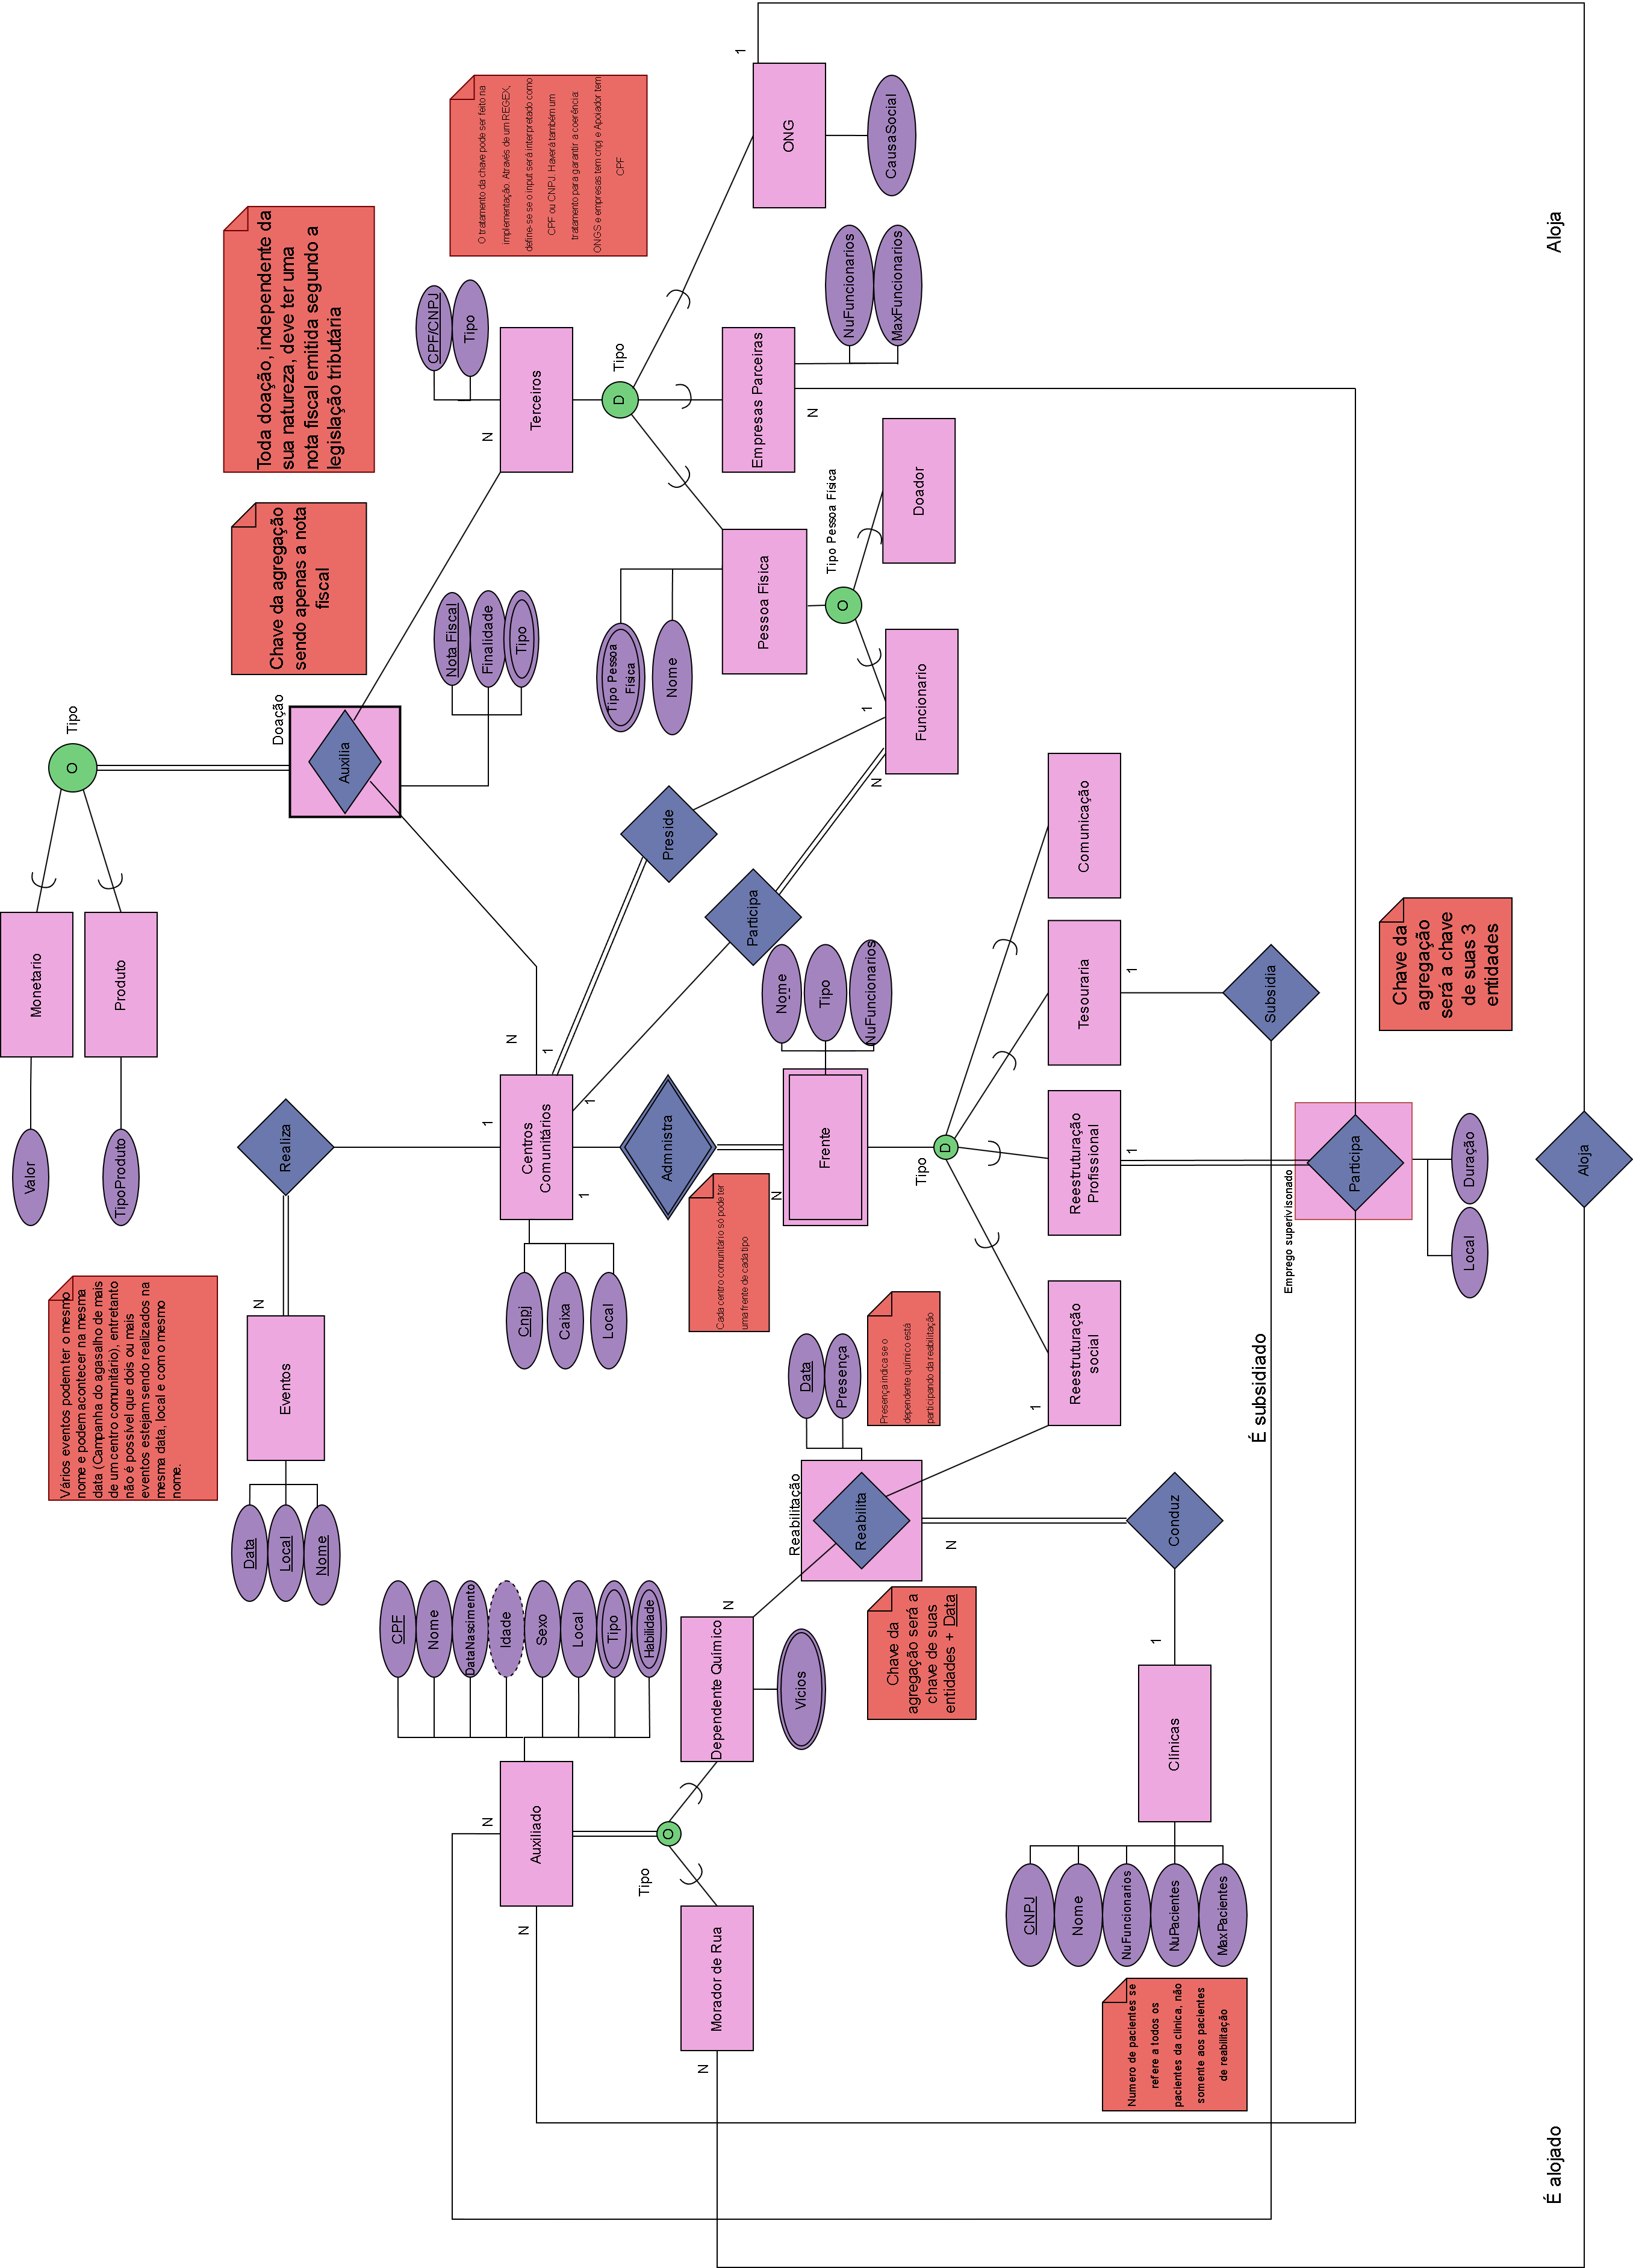
\includegraphics[scale=2]{images/Mer_VF.png}
    \label{fig:MER}
\end{figure}
\input{sections/4mudanças}
\section{Modelo Relacional}
\subsection{Imagem do Modelo Relacional}

\begin{figure}[H]
    \centering
    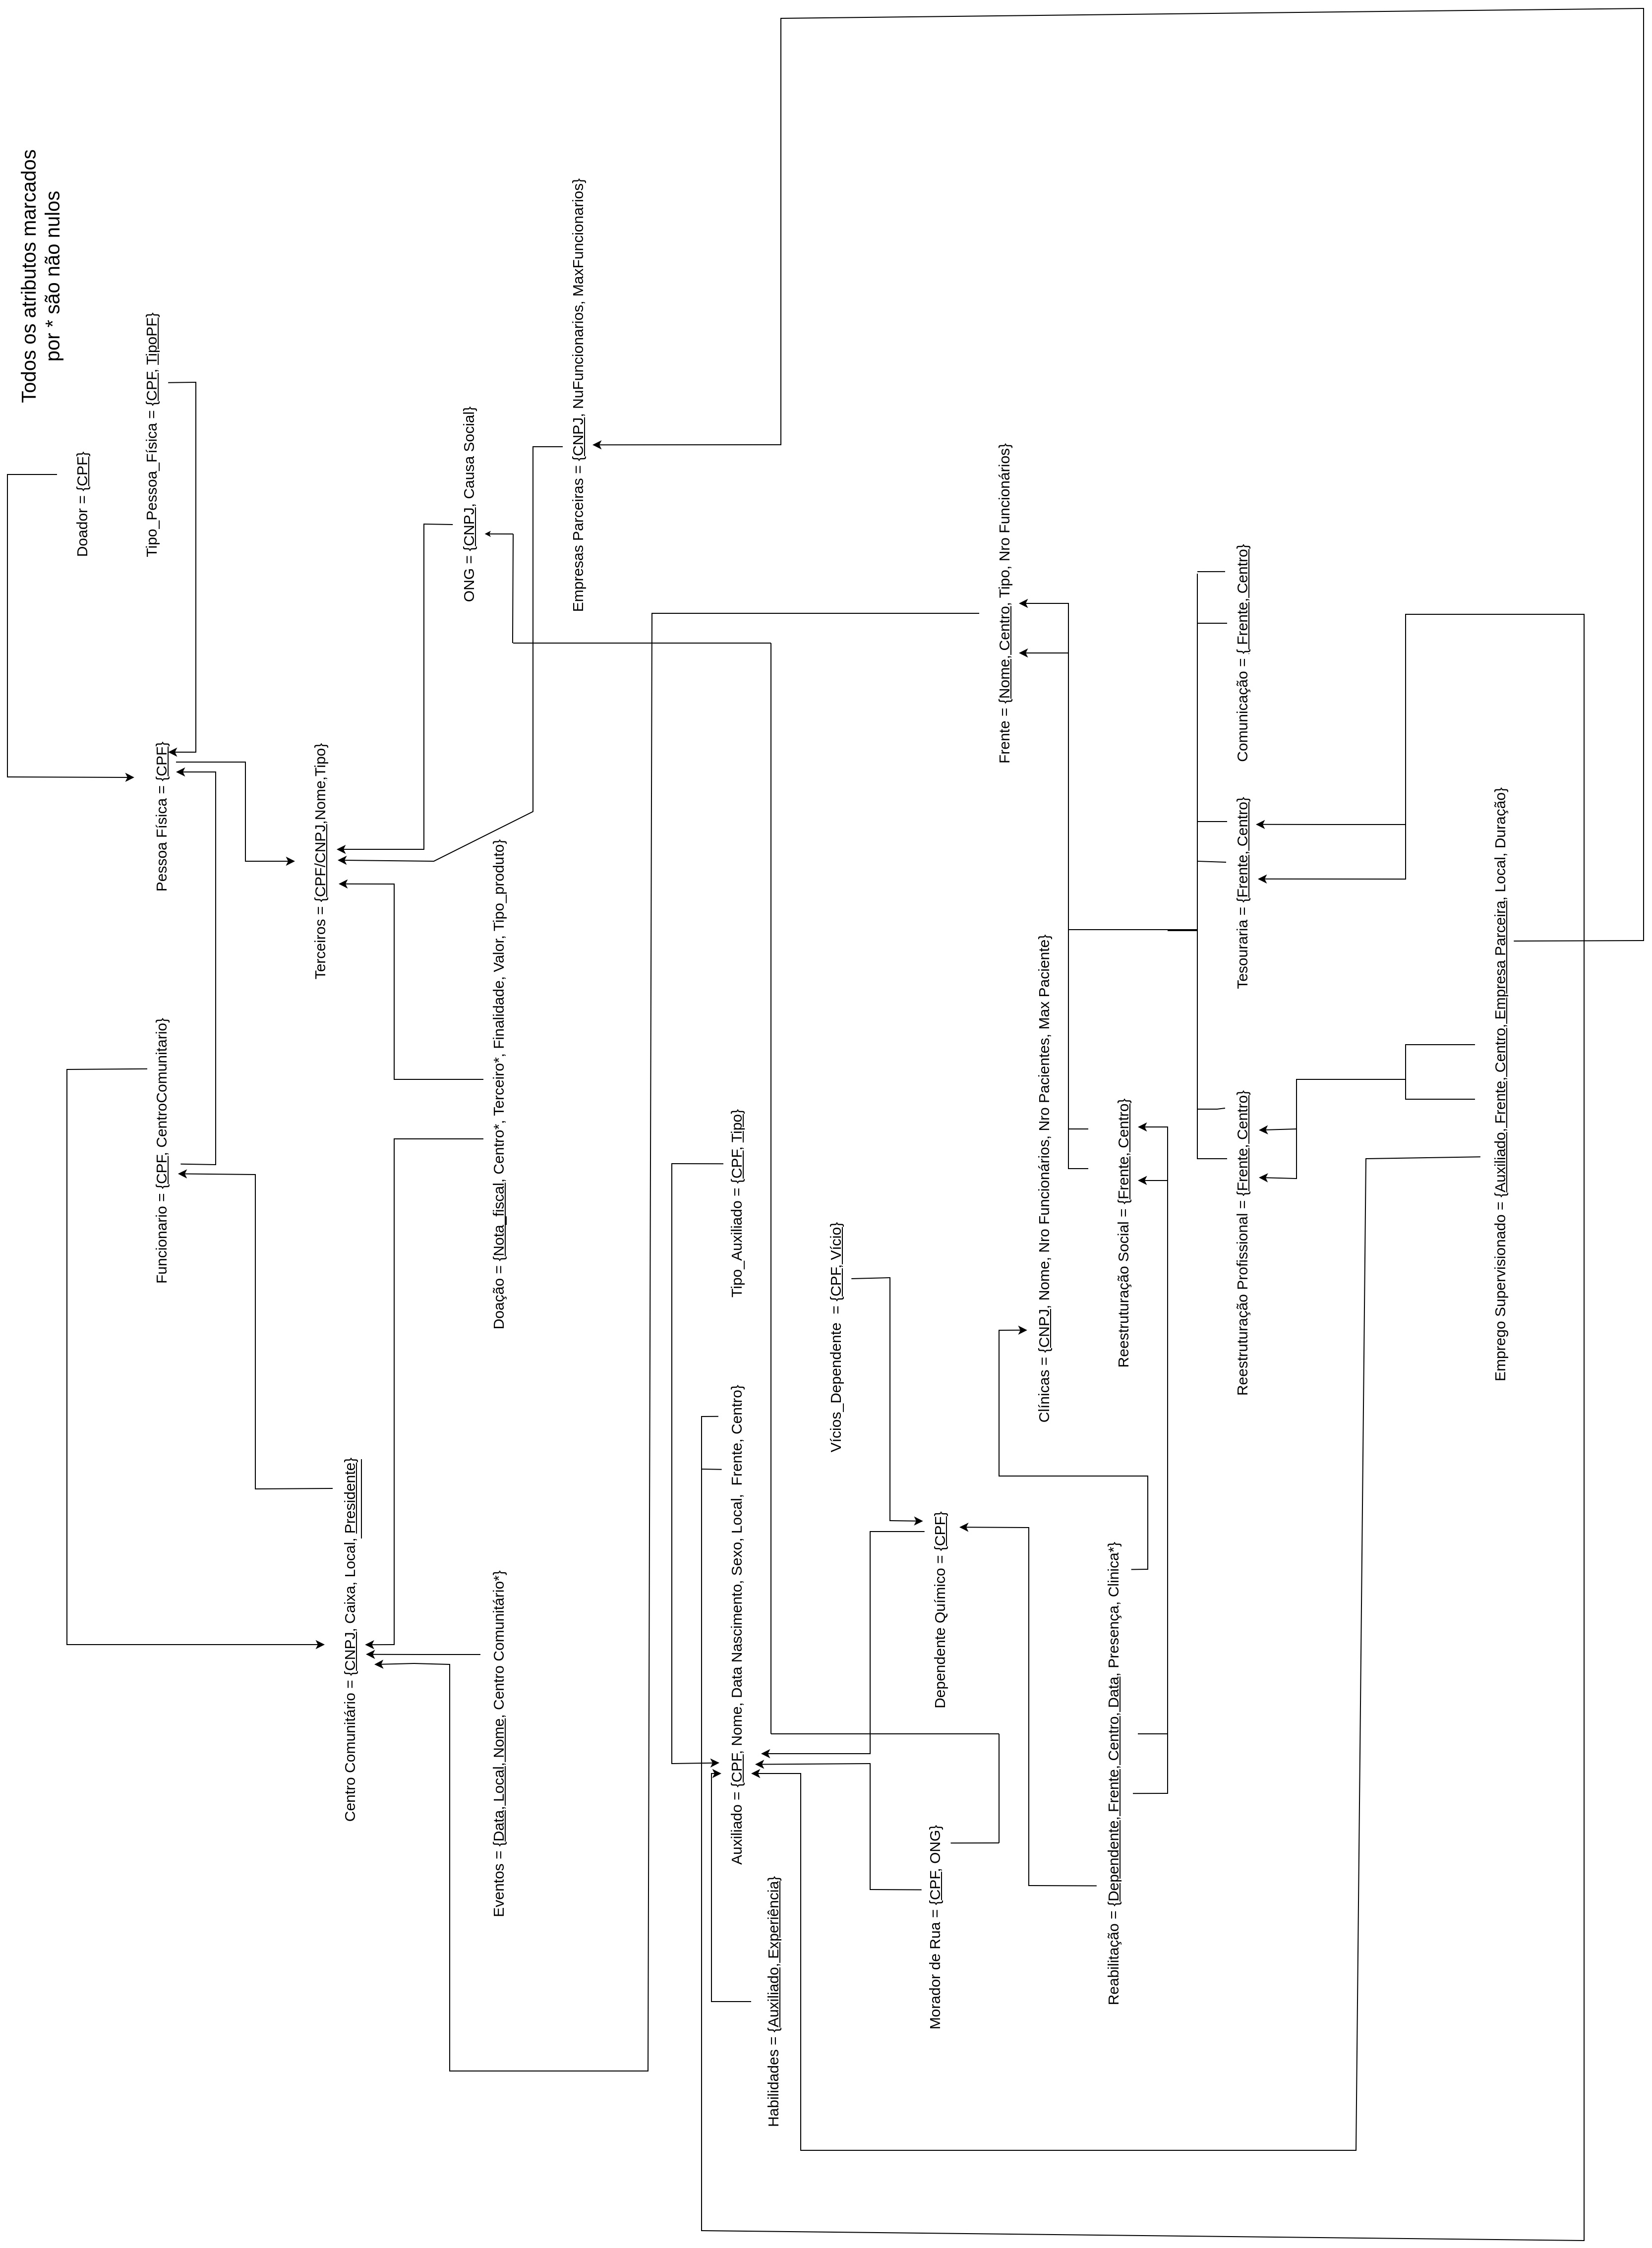
\includegraphics[scale=0.13]{images/Modelo_Relacional_VF.png}
    \label{fig:Relacional}
\end{figure}

\subsection{Restrições de integridade}
\begin{enumerate}
    \item \textbf{Possível inconsistência nas especializações totais (Doação, auxiliado)}
    
    A modelagem utilizada não garante uma especialização total dessas partes, sendo necessária atenção especial no processo de implementação.
    \item \textbf{Possível inconsistência na chave de terceiro}
    
    Como supracitado, a chave necessita ser CPF para Pessoas físicas e CNPJ para ONGS/Empresas parceiras. Nesse ponto, o tratamento ficará a cargo da implementação, sendo sugerida a utilização de RegEx em parceria com regras de entrada para garantir a funcionalidade.
    \item \textbf{Ciclo Presidente} $\xrightarrow[]{}$ \textbf{Centro comunitário}
    
    O entendimento correto desse ciclo demonstra que o Presidente de um centro comunitário deve ser um funcionário participante do mesmo.
\end{enumerate}

\subsection{Justificativas para a modelagem}
A seguir estão listadas as justificativas tomadas para a criação do modelo
relacional utilizando o modelo entidade relacionamento desenvolvido no tópico
anterior.

\begin{enumerate}

    \item \textbf{Modelagem 1:1 (Preside)}
    \\
    \textbf{Solução Adotada}: Devido a participação total, a melhor alternativa encontrada foi referenciar, dentro de centro comunitário, um presidente através de uma chave estrangeira com a presença do indicador de not null.
    \\
    \textbf{Desvantagens}: À priori, essa maneira é a ideal de representar a relação, não possuindo desvantagens evidentes.
    \\
    \textbf{Solução Alternativa}: Poderia-se criar uma tabela à parte, com tupla de centro e funcionário. Sendo centro chave primária e presidente chave secundária não nula, o efeito final seria semelhamte, mas haveria maior processamento.

    
    \item \textbf{Modelagem 1:N}
    \\
    \textbf{Solução Adotada}: Nestes casos, opta-se por modelar normalmente a entidade com cardinalidade "1" e inseri-la dentro da entidade com cardinalidade N. Em casos onde há participação total, essa inserção é acompanhada de um not null.
    \\
    \textbf{Vantagem}: Em relacionamentos com participação total, essa solução garante que esse campo nunca será nulo na hora de inserção em tabela.
    \\
    \textbf{Desvantagem}: Em situações como a relação de alojamento ou subsidia, onde não há participação total, a entidade que engloba a outra poderá conter campos vazios. Por se tratar de pouca informação, não é um empecilho realmente grande.
    \\
    \textbf{Solução Alternativa}: Poderia-se criar uma nova tabela referenciando por chave estrangeira cada uma das entidades. Contudo, trata-se de uma ação muito exagerada - devido a criação de tabela, indexação de valores - para reduzir um problema que à priori é muito pouco impactante (na parte relativa ao "Aloja"), por essa razão, opta-se pela abordagem realizada.

    \item \textbf{Mapeamento da agregação Reabilitação}
    \\
    \textbf{Solução Adotada}: Criação de uma tabela contendo as chaves da clínica, frente (que no caso, herda a também a chave de Centro, por ser entidade fraca) e do dependente químico.
    \\
    \textbf{Vantagem}: Permite a modelagem e unicidade dos tratamentos de forma idealizada, permitindo manter um controle da presença.
    \\ 
    \textbf{Desvantagens}: Como possui uma entidade fraca, o resultado final é muito sujo, por possuir muitas chaves estrangeiras.
    \\
    \textbf{Solução alternativa}: A modelagem poderia possuir um ID, reduzindo esses custos. Contudo, a presença das chaves estrangeiras torna mais semântico o entendimento da agregação e não é um impacto realmente grande a ponto de necessitar de uma troca.

    \item \textbf{Mapeamento da agregação Emprego Supervisionado }
    \\
    \textbf{Solução Adotada}: Criação de uma tabela contendo as chaves da empresa, frente (que no caso, herda a também a chave de Centro, por ser entidade fraca) e do auxiliado.
    \\
    \textbf{Vantagem}: Permite a modelagem e unicidade dos tratamentos de forma idealizada, permitindo manter um controle da atuação do auxiliado.
    \\ 
    \textbf{Desvantagens}: Como possui uma entidade fraca, o resultado final é muito sujo, por possuir muitas chaves estrangeiras.
    \\
    \textbf{Solução alternativa}: A modelagem poderia possuir um ID, reduzindo esses custos. Contudo, a presença das chaves estrangeiras torna mais semântico o entendimento da agregação e não é um impacto realmente grande a ponto de necessitar de uma troca.

    \item Mapeamento da agregação Doação
    \\
    \textbf{Solução Adotada}: Criação de uma tabela com chave primária sendo nota fiscal. Há também a referência tanto ao Centro como ao terceiro, mas à parte da chave principal.
    \\
    \textbf{Vantagem}: A utilização de uma nota fiscal aumenta a eficiência do sistema e, desta maneira, a agregação criada permite o controle de forma rápida e direcionada das doações recebidas pelo centro.
    \\ 
    \textbf{Desvantagens}: Não há.

    \textbf{Solução Alternativa}: O conjunto poderia ser identificado pelo doador, centro comunitário e data/hora, por exemplo. Contudo, a pesquisa ficaria mais lenta e não há realmente uma razão para realizar a troca de nota fiscal.

    \item \textbf{Mapeamento especialização Terceiros, Frente}:
    \\
    \textbf{Solução Adotada}: Criação de uma tabela geral, contendo a chave primária e atributos gerais. Criação de uma tabela específica, contendo os atributos específicos e, por fim, criação de uma tabela de controle, herdando a chave da entidade geral para tentar garantir seu disjoint.
    \\
    \textbf{Vantagem}: Por conta das entidades específicas possuírem relações próprias, faz-se necessário sua modelagem. A criação de uma tabela de controle facilita a busca e torna o projeto mais eficiente

    \textbf{Desvantagens}: As entidades específicas possuem poucos ou nenhum atributo próprio, tornando um pouco desperdício sua modelagem à parte. Todas elas são bem semelhantes em seus dados, podendo haver também uma repetição muito grande. Em alguns casos, com um erro por parte da inserção bem exagerado, poderia-se criar uma situação onde o Disjoint não fosse garantido. 

    \textbf{Soluções Alternativas}: A modelagem podia consistir de uma criação apenas das entidades específicas, sem a criação de uma geral. Contudo, haveria muita repetição de relacionamentos, uma vez que cada uma deveria replicar as relações da entidade geral retirada.

     \item \textbf{Mapeamento especialização Auxiliado}:
    \\
    \textbf{Solução Adotada}: Criação de uma tabela geral, contendo a chave primária e atributos gerais, bem como o atributo de especialização. Criação de uma tabela específica, contendo os atributos específicos.
    \\
    \textbf{Vantagem}: Por conta das entidades específicas possuírem relações próprias, faz-se necessário sua modelagem. Evita a criação de uma tabela extra de controle

    \textbf{Desvantagens}: As buscas podem se tornar um pouco lentas, por não se ter uma correlação direta entre Auxiliado e Tipo, como anteriormente usado na tabela de controle. Em discussão com o grupo, concluímos que essa maneira era mais limpa e valeria a pena mesmo assim. Não garante também a especialização total. 

    \textbf{Soluções Alternativas}: A modelagem poderia seguir os padrões anteriores, utilizando uma tabela de controle. No fim, a indexação talvez não fizesse valer a pena, haja vista que essa consulta além de não ser tão utilizada, não fica lenta o suficiente na modelagem usada para ser necessário sua mudança.
    
    
    \item \textbf{Mapeamento da especialização Doação}
    \\
    \textbf{Solução Adotada}: Unificação de todos os atributos das entidades específicas na tabela única doação.
    \\
    \textbf{Vantagem}: A utilização de menos tabelas faz com que o tempo de busca seja favorecido, pois não será necessário acessar duas tabelas distintas e é diminuído o tamanho em armazenamento da base de dados.
    \\ 
    \textbf{Desvantagens}: Pode gerar muitos valores nulos caso várias doações de apenas um tipo, monetária ou de produto, sejam realizadas.

    \textbf{Solução Alternativa}: Construir uma tabela para cada entidade específica, possuindo uma chave estrangeira como chave principal, a qual seria o número de nota fiscal da doação referente, além de uma tabela para categorizar os tipos, também tendo o número da nota fiscal como chave estrangeira e chave primária da tabela, que é composta com tipo.

    \item \textbf{Mapeamento da especialização Pessoa Física}
    \\
    \textbf{Solução Adotada}: Criação de uma tabela geral, contendo a chave primária e atributos gerais, bem como o atributo de especialização. Criação de uma tabela específica, contendo os atributos específicos. 
    \\
    \textbf{Vantagem}: Por conta das entidades específicas possuírem relações próprias, faz-se necessário sua modelagem. Evita a criação de uma tabela extra de controle, melhorando o tempo no quesito de indexação.

    \textbf{Desvantagens}: As buscas podem se tornar um pouco lentas, por não se ter uma correlação direta entre Pessoa Física e Tipo, como anteriormente usado na tabela de controle. Por não ser necessário especialização total, é uma boa abordagem.

    \textbf{Soluções Alternativas}: A modelagem poderia seguir os padrões anteriores, utilizando uma tabela de controle. No fim, a indexação talvez não fizesse valer a pena, haja vista que essa consulta além de não ser tão utilizada, não fica lenta o suficiente na modelagem usada para ser necessário sua mudança.
    
    \item \textbf{Atributos Multivalorados (Vícios, Habilidades)}:
    \textbf{Solução Adotada}: Seguiu-se a modelagem padrão para atributos multivalorados, onde cria-se uma tabela, herdando a chave principal de sua entidade-mãe que fará parte da chave primária da próxima tabela, juntamente com o seu diferenciador. Por exemplo, para a tabela de vícios, as chaves serão compostas pelo CPF do auxiliado, bem como pelo vício em si. De forma análoga para as habilidades, onde a tabela de habilidades possuirá o CPF do indivíduo e, para cada habilidade, será gerada uma nova tupla.
    \\
    \textbf{Vantagem}: A modelagem facilita a correlação dos valores, sendo amplamente utilizada para essas situações.

    \textbf{Desvantagens}: Pode-se ter valores nulos e o processo de indexação em si consome processamento.

    \textbf{Soluções Alternativas}: Dependendo da importância dada à estes pontos, como trata-se de atributos multivalorados, caso eles sejam considerados descartáveis, poderiam ser apresentados como uma grande string univalorada. Futuramente, em tratamento de aplicação, através de um parser, esses valores poderiam ser retornados.
    
    
    \item \textbf{Mapeamento do atributo derivado `idade` da entidade `Auxiliado`}
    
    \textbf{Solução adotada:} O atributo `idade` da entidade `Auxiliado` foi mapeado como sendo derivado por seu baixo custo de calculo e para evitar colocar informações redundantes no modelo. Portanto, como foi considerado atributo derivado ele não foi colocado na tabela `auxiliado` no modelo relacional.
    \\
    \textbf{Vantagens: } Diminui a quantidade de dados armazenados nesta entidade. 
    \\
    \textbf{Desvantagens: } O cálculo que é necessário para ter a informação do atributo, desacelera possíveis tratamentos.
    \\
    \textbf{Soluções Alternativas: } Colocar o atributo não sendo derivado. Isso implicaria que todos os dias um cálculo deverá ser feito para todas os membros daquela entidade, o que pode ser custoso de acordo com o tamanho da entidade.
    
\end{enumerate}
\input{sections/6mudanças.tex}
\section{Implementação}
Nesta seção serão definidas as minucias que permeiam nossa aplicação, a qual foi implementada utilizando a linguagem de programação Python na versão estável 3.10.8 para as interfaces gráficas e interativas e para administrar nosso banco de dados foi empregado o SGBD (Sistema de Gerenciamento de Banco de Dados) foi utilizado o PostgreSQL, a integração e composição entre ambos foi feita utilizando o Docker e o driver Psycopg.

A aplicação consiste de um ambiente interativo que permite a realização de consultas pré-especificadas que serão expostas em maiores detalhes, e a realização de consultas personalizadas de acordo com a necessidade do usuário, dentre queries pré-estabelecidas. A interface de usuário foi feita baseada na biblioteca CustomTkinter, externa a linguagem de programação Python.
\subsection{Script de Consultas}

Os dados utilizados para as consultas (esquema, dados e consultas) pode ser encontrado no repositório da implementação, na pasta "data", \href{https://github.com/Franreno/AuxilioDepQuim/tree/main/data}{neste link}.


\lstset{language=SQL,
             basicstyle=\footnotesize,
             numbers=left,
             numberstyle=\footnotesize,
             frame=shadowbox,
             rulesepcolor=\color{red}}
\begin{itemize}
    \item \textbf{C1-Consultar informações do auxiliado referentes a sua reabilitação}
    
    \begin{lstlisting}
        SELECT A.NOME,C.NOME,R.PRESENCA 
        FROM REABILITACAO R 
        JOIN AUXILIADO A 
        ON R.DEPENDENTE = A.CPF 
        JOIN CLINICA C 
        ON R.CLINICA = C.CNPJ 
        WHERE(SELECT AVG(R1.PRESENCA) FROM REABILITACAO R1) < R.PRESENCA;  
    \end{lstlisting}
    
    Nesta consulta foi realizado o \textit{inner join} das tabelas REABILITACAO, AUXILIADO e CLINICA, a fim de extrair de cada uma delas o nome do AUXILIADO, a CLINICA que ele está em REABILITACAO e sua presença. A junção é realizada garantindo que só serão expostos auxiliados cujo a presença seja maior que a média geral de todos os auxiliados, isso é garantido pelas cláusulas ON presentes na consulta, que garantem a junção apenas de tuplas que atendam aos requisitos da cláusula WHERE.

    \item \textbf{C2-Consulta de empresas parceiras com vagas de emprego supervisionado}

    \begin{lstlisting}
        SELECT T.NOME, EP.NUFUNCIONARIOS, ES.LOCAL
        FROM TERCEIROS T
        JOIN EMPREGO_SUPERVISIONADO ES
        ON T.NUCPFCNPJ = ES.EMPRESA_PARCEIRA
        JOIN EMPRESAS_PARCEIRAS EP
        ON ES.EMPRESA_PARCEIRA = EP.CNPJ
        WHERE EP.MAXFUNCIONARIOS > EP.NUFUNCIONARIOS;
    \end{lstlisting}

    Neste procedimento são selecionados nome, número de funcionários trabalhando atualmente e local da vaga oferecida referentes a uma empresa parceira, estas informações estão presentes, respectivamente, nas tabelas TERCEIROS, EMPRESAS\_PARCEIRAS E EMPREGO\_SUPERVISIONADO. Como as informações que buscamos estão em tabelas distintas é utilizada a junção interna, representada em SQL pela cláusula JOIN, a garantia de coerência e objetividade das informações buscadas são garantidas pelas cláusulas ON, a qual realiza a junção apenas das tuplas que atendem as demandas feitas em WHERE e propaga isso de forma encadeada. A clausula WHERE garante que as tuplas selecionadas em EMPRESAS\_PARCEIRAS tenham um número máximo de funcionários maior que o número que já ocupa as vagas, i.e, pode receber novos trabalhadores.

    \item \textbf{C3-Consulta do status empregatício de um auxiliado} 
    
    \begin{lstlisting}
        SELECT A.NOME,
        CASE 
            WHEN  ES.DURACAO - CURRENT_DATE < 10 
            AND ES.DURACAO - CURRENT_DATE > 0
                THEN 'PROXIMO AO FIM'
            WHEN ES.DURACAO- CURRENT_DATE > 10 
                THEN 'FUNCIONARIO EMPREGADO'
            WHEN (ES.DURACAO - CURRENT_DATE < 0) 
            OR ES.DURACAO IS NULL
                THEN 'FUNCIONARIO DESEMPREGADO'
            END STATUS_EMPREGO
        FROM AUXILIADO A
        LEFT JOIN EMPREGO_SUPERVISIONADO ES
        ON A.CPF = ES.AUXILIADO
        LEFT JOIN TERCEIROS E
        ON ES.EMPRESA_PARCEIRA = E.NUCPFCNPJ;
    \end{lstlisting}

    Nesta consulta são retornadas tuplas com o nome do auxiliado associado ao seu status empregatício, baseado em uma subtração entre a duração do emprego supervisionado e a data atual. Isso foi feito através da cláusula CASE que pode classificar através da diretiva WHEN. Na aplicação, se o auxiliado tem menos de dez dias de emprego supervisionado planejados, é considerado que seu trabalho está PROXIMO AO FIM, caso contrário ele tem o status de FUNCIONARIO EMPREGADO caso tenha mais de dez dias até o fim de seu contrato ou está desempregado caso o atributo DURACAO seja nulo ou apresente uma data menor que a data atual.

    \item \textbf{C4-Consulta de todos os auxiliados empregados}

    \begin{lstlisting}
        SELECT * from AUXILIADO A
        JOIN EMPREGO_SUPERVISIONADO ES
        ON A.CPF = ES.AUXILIADO;
    \end{lstlisting}

    Nesta consulta nos interessa recuperar todas as tuplas de auxiliados que estão relacionadas a um emprego supervisionado, i.e, nos interessa saber quais auxiliados estão empregados e suas informações. O retorno apenas das tuplas da tabela AUXILIADO referentes a participantes com emprego ativo é garantido pela junção interna, representada pela cláusula JOIN em conjunto com a clásula ON, a qual delimita as tuplas de acordo com a condição apresentada. 

    \item \textbf{C5-Consulta de centros e de quantos auxiliados se beneficiam de sua tesouraria}

    \begin{lstlisting}
        SELECT C.NOME, COUNT(*) FROM
        CENTRO C JOIN TESOURARIA T
        ON C.CNPJ = T.CENTRO
        JOIN AUXILIADO A  
        ON A.FRENTE = T.FRENTE AND  T.CENTRO = A.CENTRO
        GROUP BY C.NOME;
    \end{lstlisting}

    Nesta consulta são retornadas as tuplas contendo os nomes de todos os centro que possuem tesouraria e quantos auxiliados são subsidiados pelas suas respectivas tesourarias. Nesta consulta foi utilizada a cláusula GROUP BY para realizar a contagem da quantidade de tuplas referente a grupos separados pelo nome dos centros selecionados. Além disso, as cláusulas JOIN associadas as cláusulas ON garantem que são selecionados apenas centros com tesourarias na primeira afirmação lógica, destas são segregadas apenas as tesourarias que possuem auxiliados na segunda afirmação lógica, por fim os centros comunitários são agrupados pelos seus respectivos nomes.

    \item \textbf{C6-Consulta os auxiliados que são apenas moradores de rua}

    \begin{lstlisting}
        SELECT A.NOME, A.LOCAL FROM
        AUXILIADO A JOIN TIPO_AUXILIADO TA
        ON A.CPF = TA.CPF
        WHERE A.CPF NOT IN
        (SELECT DISTINCT A.CPF FROM 
            AUXILIADO A JOIN TIPO_AUXILIADO TA
            ON A.CPF = TA.CPF
            WHERE UPPER(TA.TIPO) = 'DEPENDENTE_QUIMICO');
    \end{lstlisting}

    Nesta seleção são retornadas tuplas com nome e local dos auxiliados que são, exclusivamente, moradores de rua. A exclusividade do tipo de auxiliado vem da cláusula WHERE acompanhada de NOT IN, que não inclui os auxiliados cujo tipo é DEPENDENTE\_QUIMICO, a cláusula DISTINCT apenas evita repetições de tuplas selecionadas pela cláusula WHERE e garante otimização.
    
\end{itemize}
\subsection{Aplicação}

O repositório da aplicação pode ser encontrado \href{https://github.com/Franreno/AuxilioDepQuim}{neste link}.

\subsubsection{Requisitos do Sistema}
Além da linguagem de programação Python devidamente instalada em versão 3.8.2 ou maior é necessário instalar as dependências e o \textit{package manager} Pip referente a esta versão.

Todas as considerações feitas a seguir consideram que o usuário está utilizando um sistema operacional do tipo Linux baseado em Debian.

Para facilitar o uso da aplicação foram criados \textit{scripts} para instalação de algumas dependências, portanto é necessário estar no diretório raiz do projeto e permitir que os \textit{scripts} sejam executados através do seguinte comando no terminal:

\lstset{language=bash,
             basicstyle=\footnotesize,
             numbers=none,
             frame=shadowbox,
             rulesepcolor=\color{red}}

\begin{lstlisting}
    sudo chmod +x scripts/*.sh
\end{lstlisting}

Os pacotes Tkinter utilizado para construção da interface gráfica e Psycopg2 para integração com o PostreSQL tem como dependências os pacotes python-tk e libpq-dev respectivamente, para baixa-los basta utilizar o seguinte comando em sua shell:

\begin{lstlisting}
    sudo apt install python-tk libpq-dev
\end{lstlisting}

Para finalizar os pacotes basta baixa-los utilizando o administrador de pacotes nativo do Python, o pip, através de um arquivo de texto criado por comodidade e facilidade de uso:

\begin{lstlisting}
    pip install -r requirements.txt
\end{lstlisting}

Por fim, para realizar a instalação e a inicialização do Docker, ambiente de integração entre Python e o SGBD utilizado, basta realizar o seguinte comando em sua própria shell:

\begin{lstlisting}
    sudo scripts/install_docker_ubuntu.sh && sudo scripts/install.sh
\end{lstlisting}
\subsubsection{Funcionamento geral}
A fim de executar o programa basta utilizar o seguinte comando:

\begin{lstlisting}
    python src/main.py
\end{lstlisting}

Com isso, será exibida a interface vista na Figura \ref{fig:interface}, nela são perceptíveis os botões responsivos ao clique a esquerda, os quais desempenham as seguintes funções:
\begin{itemize}
    \item \textbf{Mostrar tabela}: É exibido um botão no estilo \textit{dropdown} contendo como opções todas as tabelas implementadas, ao selecionar uma tabela específica, são exibidas sua colunas, o tipo de cada uma e seu respectivo tamanho. É possível ver um exemplo da interface na Figura \ref{fig:mostratab}.
    \item \textbf{Rodar/Debugar SQL}: Permite a inserção direta de queries SQL através de uma interface de escrita, esta função está implementada única e exclusivamente para facilitar testes e correções e não estaria disponível ao usuário final. Funciona basicamente como um SQL injection liberado e implementado pelo sistema. Sua execução está referenciada pela Figura \ref{fig:rodarsql}, onde é possível ver uma janela inferior interativa, a qual recebe as queries, e uma janela superior, responsável por exibir os resultados.
    \item \textbf{Rodar consultas.sql}: Realiza as consultas previstas no arquivo pré-estabelecido pelos desenvolvedores. Sua execução está exposta na Figura\ref{fig:consultassql}, que exibe uma janela superior para o resultado das consultas.
    \item \textbf{Cadastrar novo funcionário, cadastrar empresa e inserir centro}: São funcionalidades de inserção de tuplas e possuem interfaces semelhantes, nessas são exibidos os atributos de cada tabela referenciada(Funcionário, Empresa Parceira e Centro Comunitário), os quais possuem um pequeno espaço para serem preenchidos os valores e um botão para confirmar a inserção. A interface referente a Cadastrar novo funcionário, que serve como base para as demais, está explicitada na Figura \ref{fig:novofunc}.
    \item \textbf{Mostrar informações}: É exibido um botão no estilo \textit{dropdown} com todas as tabelas possíveis e disponíveis para consulta, ao selecionar uma tabela é exibido um segundo botão \textit{dropdown} contendo todos os atributos da tabela, assim é possível conferir, por exemplo, todos os nomes dos auxiliados inseridos. A interface de uso pode ser vista na Figura \ref{fig:mostrarInfo}, já com os dois botões \textit{dropdown} exibidos.
\end{itemize}

Vale ressaltar que nas funcionalidades de inserção as strings inseridas nos campos delimitados são passadas como parâmetros de funções secundárias e não uma simples concatenação de strings, evitando ataques maliciosos.

\begin{figure}[H]
    \centering
    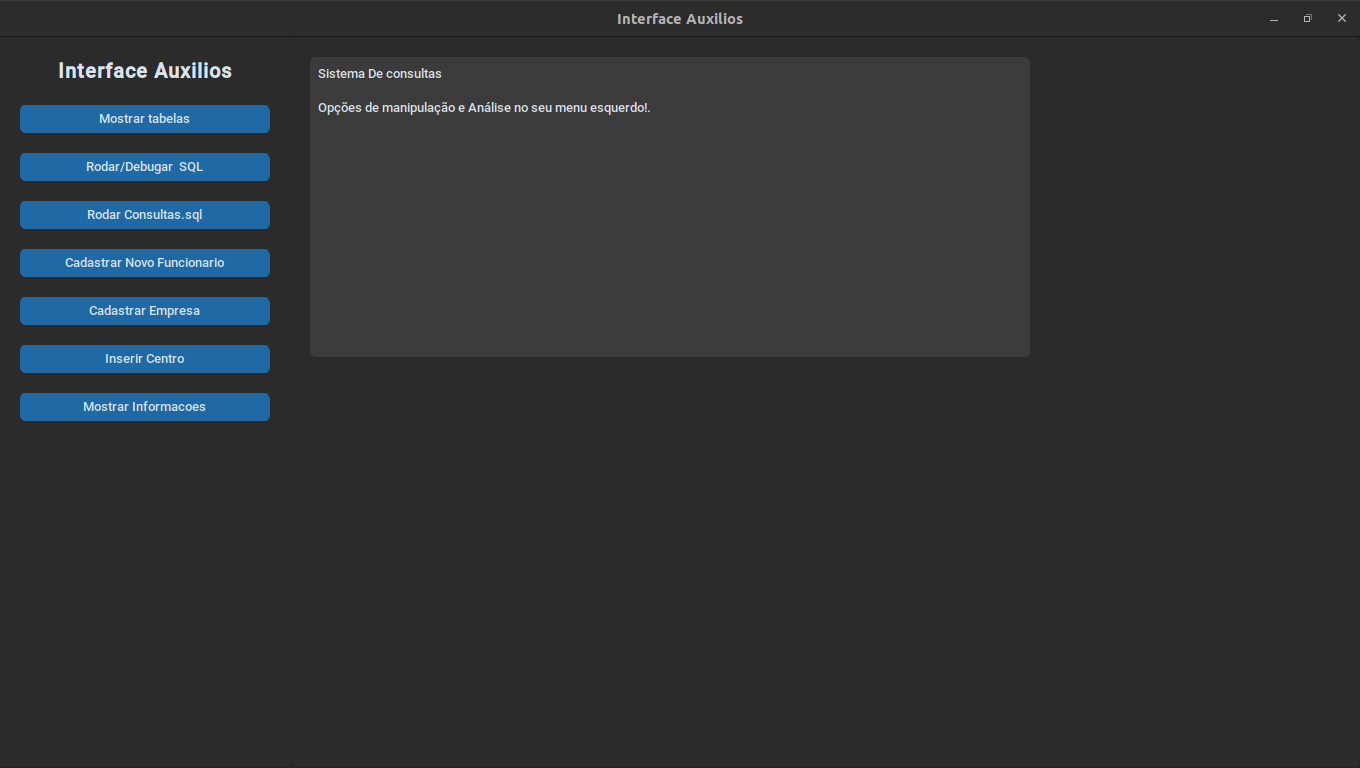
\includegraphics[scale=0.3]{images/interface.png}
    \caption{Interface inicial. \textbf{Fonte:} Autores}
    \label{fig:interface}
\end{figure}

\begin{figure}[H]
    \centering
    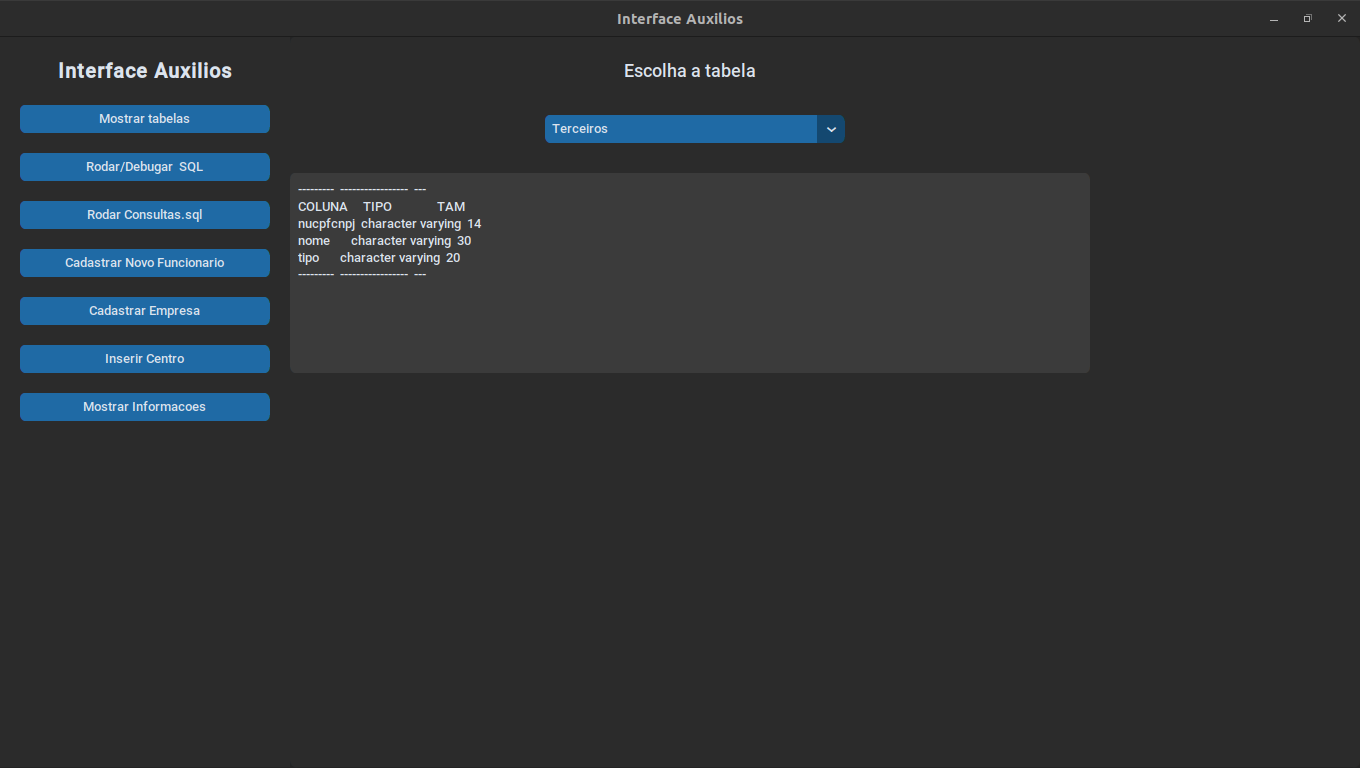
\includegraphics[scale=0.3]{images/mostratab.png}
    \caption{Interface ao selecionar o botão Mostrar tabela. \textbf{Fonte:} Autores}
    \label{fig:mostratab}
\end{figure}

\begin{figure}[H]
    \centering
    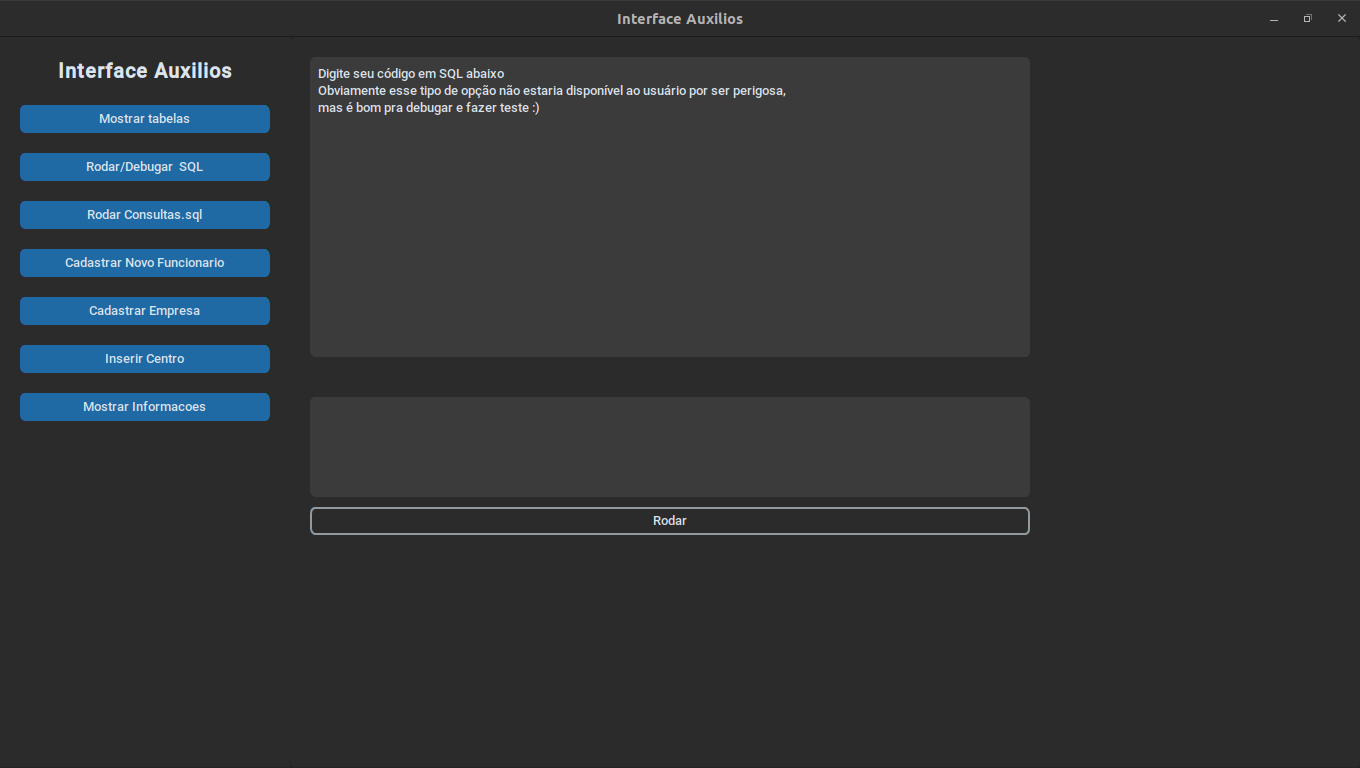
\includegraphics[scale=0.3]{images/rodarsql.png}
    \caption{Interface ao selecionar o botão Rodar/Debugar SQL. \textbf{Fonte:} Autores}
    \label{fig:rodarsql}
\end{figure}

\begin{figure}[H]
    \centering
    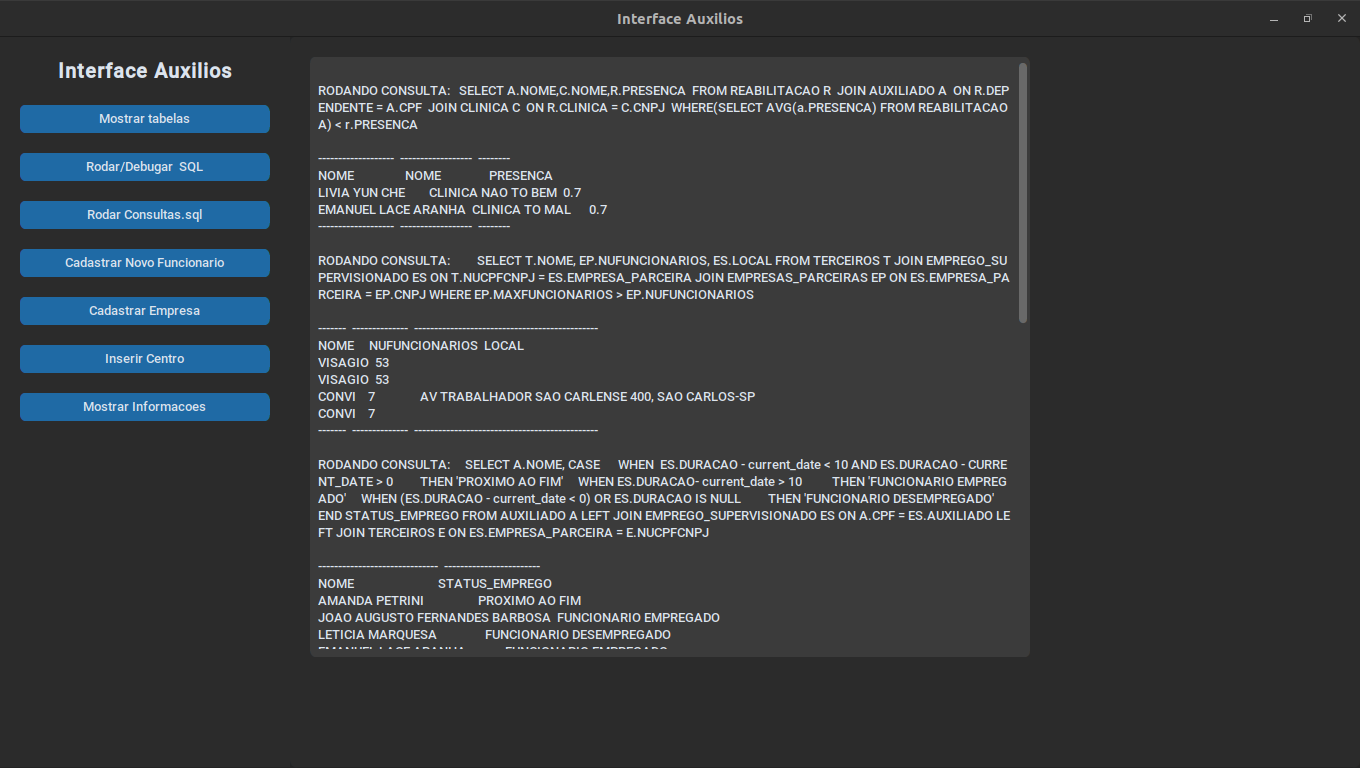
\includegraphics[scale=0.3]{images/consultassql.png}
    \caption{Interface ao selecionar o botão Rodar consultas.sql. \textbf{Fonte:} Autores}
    \label{fig:consultassql}
\end{figure}

\begin{figure}[H]
    \centering
    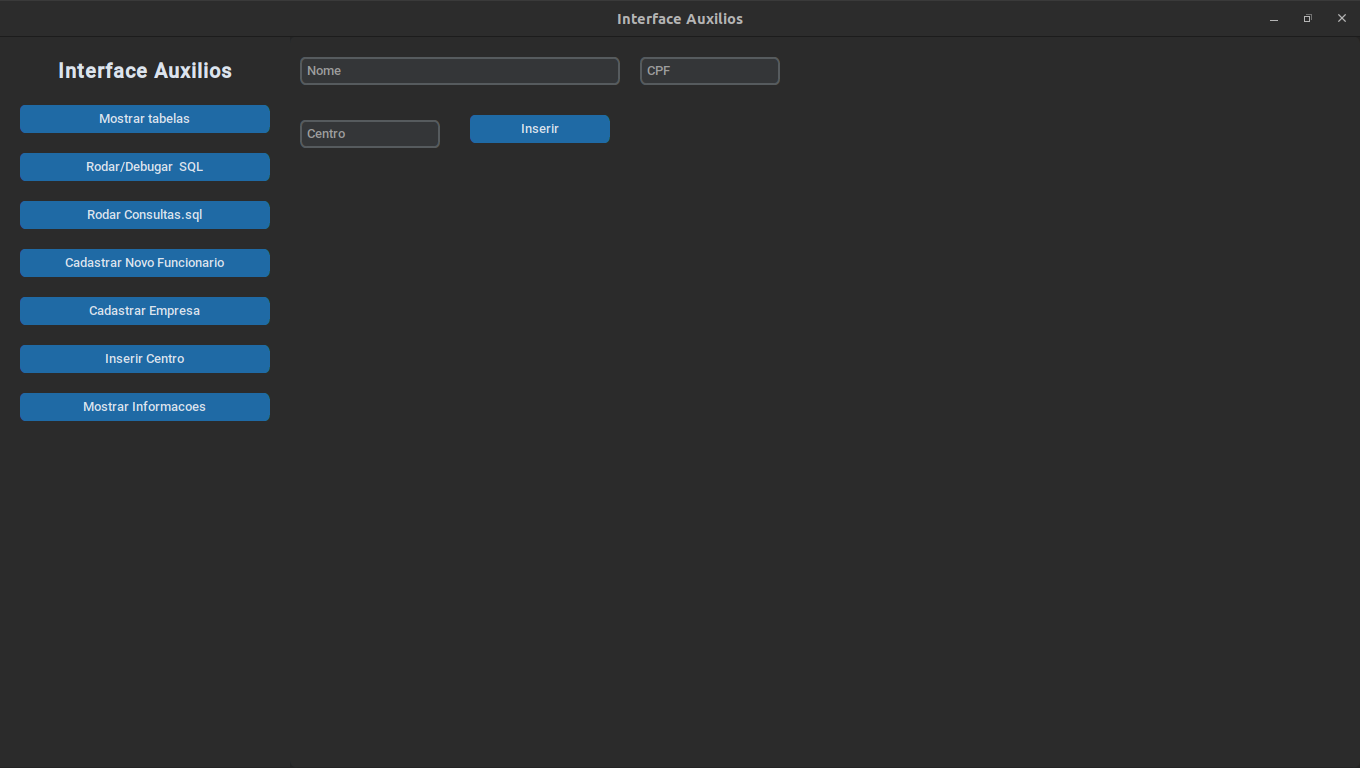
\includegraphics[scale=0.3]{images/novofunc.png}
    \caption{Interface ao selecionar o botão Cadastrar novo funcionário. \textbf{Fonte:} Autores}
    \label{fig:novofunc}
\end{figure}

\begin{figure}[H]
    \centering
    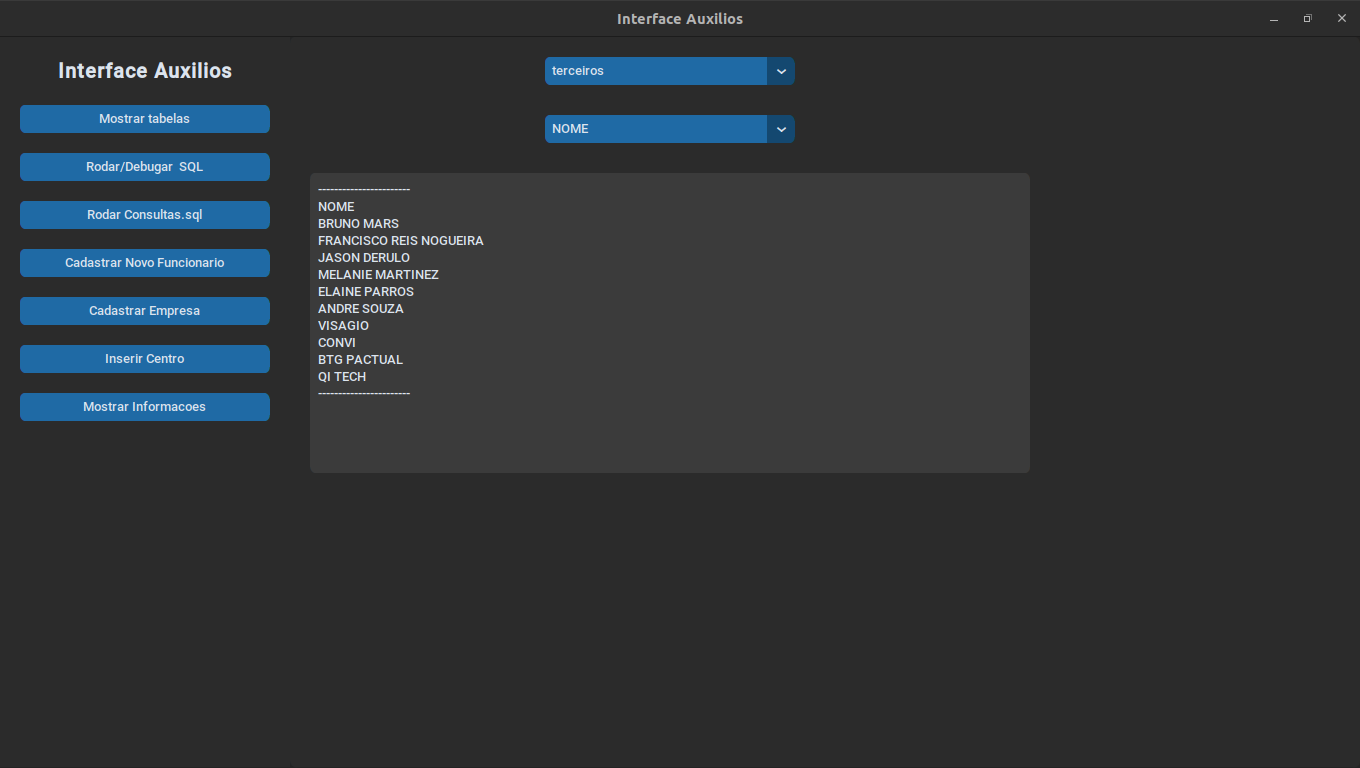
\includegraphics[scale=0.3]{images/mostrarInfo.png}
    \caption{Interface ao selecionar o botão Mostrar informações. \textbf{Fonte:} Autores}
    \label{fig:mostrarInfo}
\end{figure}


\input{sections/8Conclusão.tex}


% se quiser que as referências fiquem na mesma página da conclusão, coloque % na linha a seguir
\newpage

%\bibliographystyle{abnt-alf}
%\renewcommand{\refname}{REFERÊNCIAS BIBLIOGRÁFICAS}
%\nocite{*}
%\bibliography{biblio_rel}


\end{document}